\section{Git and GitHub}
In this project, we used GitHub to host our report LaTeX code, and the source code for our flutter application.
We have used Git to interact with GitHub and push and pull code. 

GitHub is also linked to our Azure Pipelines as described in~\autoref{azurepipelines}.

We use the principles of Gitflow, that requires developers to create a branch for each new feature, hot fixes and bug fixes. 
The branches can then be merged back into their respective branches when the branch is completed.
This is done using pull requests, which has to be approved by at least one other developer.
This ensures that no code is merged into the main branches, with approval of at least one other developer.

\begin{figure}[H]
    \centering
    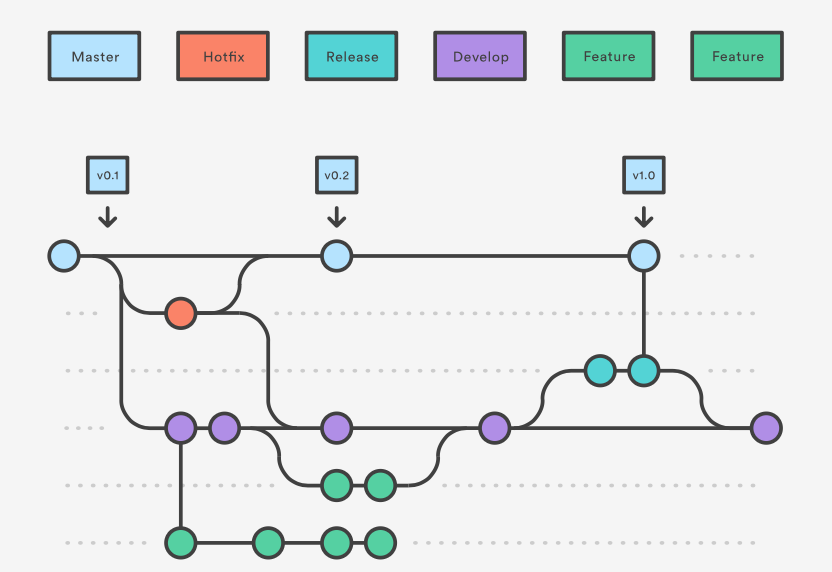
\includegraphics[width=0.8\textwidth]{images/GitFlow.png}
    \caption{Gitflow diagram, showing how branches should be created and named.}
    \label{Gitflow}
\end{figure}


\subsection{Git and GitHub within the application}
As software developers ourselves, we have used GitHub and love it.
However some product owners will have very limited or no experience at all with Git or GitHub.
We thought if the issues could be made directly by the product owner, it would make it easier for the developers to keep track is
This is where our product comes to the rescue.
It allows any product owner with no Git or GitHub experience, to create issues and tasks for developers to use.